%%%%%%%%%%%%%%%%%%%%%%%%%%%%%%%%%%%%%%%%%%%%%%%%%%%%%%%%%%%%%%%%%%%%%
%                                                                   %
%	CHAPTER THREE, SOFTWARE AND API                                   %
%                                                                   %
%%%%%%%%%%%%%%%%%%%%%%%%%%%%%%%%%%%%%%%%%%%%%%%%%%%%%%%%%%%%%%%%%%%%%

\chapter{Runtimes, Software, API and Benchmarks}

\section{Introduction}
After presenting the rules of HPC and the hardware that compose the cluster we need to introduice ways to target this supercomputer. 
Several options are present in the language, the multi-processing API, the distribution and the accelerators code. 
This chapter details the most important software options for HPC programming and include the choices we made for our applications.

Then it presents the software used to benchmark the supercomputers. 
We present here the most famous, the TOP500, GRAPH500 and GREEN500 to give their advantages and weaknesses. 

\todo{Parler des pitfalls, load balancing, concurrence, ... or when the case.}

\section{Sofware/API}
In this section we present the main runtimes, API and programming language use in HPC and in this study in particular. 
The considered language will be C/C++, the most present in HPC world.

\subsection{Parallel programming}

\subsubsection{PThreads}
The POSIX threads API is an execution model available in most of the languages. 
It allows the user to define threads that will execute concurrently on the processor ressources using shared/private memory.
PThreads is the low level handling of threads and the user need to handle concurrency with mutex, conditions variables and synchronization "by hand".
This makes the PThreads hard to use in complex applications and used only for very fine-grained control over the threads management. 
\todo{Fine-grain Coarse-grain applications}

\subsubsection{OpenMP}
Open Multi-Processing, OpenMP\footnote{http://www.openmp.org}~\cite{chapman2008using,supinski2017scaling}, is an API for multi-processing shared memory like UMA and CC-NUMA.
It is available in C/C++ and Fortran.
The user is provided with pragmas and functions to declare parallel loop and regions in the code. 
In this model the main thread, the first one before forks, command the fork-join operations. 

The last versions of OpenMP also allow the user to target accelerators. 
During compilation the user specify on which processor or accelerator the code will be executed in parallel. 

\subsubsection{Ohters}
Many other tools handle parallel programming for processors.
Cilk for C/C++ base, like OpenMP, on Fork-Join paradm. 
Threads Building Blocks, TBB, from Intel.

\subsection{Distributed programming}
In the cluster once the code have been developped locally and using the multiple cores available, the new step is to distribute it all over the nodes of the cluster. 
This step requires the processes to access NoRMA memory from a node to another. 
Several runtime are possible for this purpose.

\subsubsection{MPI}
The Message Passing Interface, MPI, is the most and widely spread runtime for distributed computing~\cite{gropp2014using,gropp2015using}.
Several implementations exists from Intel MPI\footnote{https://software.intel.com/en-us/intel-mpi-library} (IMPI), MVAPICH\footnote{http://mvapich.cse.ohio-state.edu/} by the Ohio State University and OpenMP\footnote{http://www.open-mpi.org} combining several MPI work like Los Alamos MPI (LA-MPI).
Those implementation follow the MPI standards 1.0, 2.0 or the latest, 3.0. 
\todo{Who define standards ??}

Some MPI implementation offer a support for accelerators targeting directly their memory through the network without multiple copies on host memory. 

\subsubsection{Charm++}
Charm++\footnote{http://charmplusplus.org/} is another API for distributed programming developped by the University of Illinois Urbana-Champaign.
It is asynchronous messages paradigm driven.
In contrary of runtime like MPI that are synchronous but can handle asynchronous, charm++ is natively asynchronous. 
It is based on \textit{chare object} that can be activated in response to messages from other \textit{chare objects} with actions and callbacks. 
The repartition of data to processors is completely done by the API, the user just have to define correctly the partition of the program. 
Charm++ also provide a GPU manager implementing data movement, asynchronous kernel launch, callbacks, etc.

A perfect example can be the hydrodynamics N-body simulation code Charm++ N-body Gravity Solver, ChaNGa~\cite{jetley2010scaling}, implemented with charm++ and GPU support. 

\subsubsection{Legion}
The Legion\footnote{http://legion.stanford.edu/} is a distributed runtime support but Stanford University, Los Alamos National Laboratory and NVIDIA. 
This runtime is data-centered targeting distributed heterogeneous architectures. 
Data-centered runtime focus to keep the data dependency and locality moving the tasks to the data and moving data only if requested. 
In this runtime the user define data organization, partitions, priviledges and coherence. 
Many aspect of the distribution and parallelization are then handle by the runtime itself.

\subsection{Other tools}
HPX ? 
Others ? 

\subsection{Accelerators}
\subsubsection{CUDA}
The Compute Device Unified Architecture is the API develop in C/C++ Fortran by NVIDIA to target its GPGPUs. 
The API provide high and low level functions. 
The driver API allows a fine grain control over the executions.

The CUDA compiler is called NVdia C Compiler, NVCC. 
It converts the device code into Parallel Thread eXecution, PTX, and rely to the C++ host compiler for host code. 
PTX is a pseudo assembly language translated by the GPU in binary code that is then execute. 
As the ISA is pretty simple it able the user to work directly in assembly for very fine grain optimizations. 

\subsubsection{OpenCL}

\todo{Section for profiling?}

\begin{figure}
\centering 
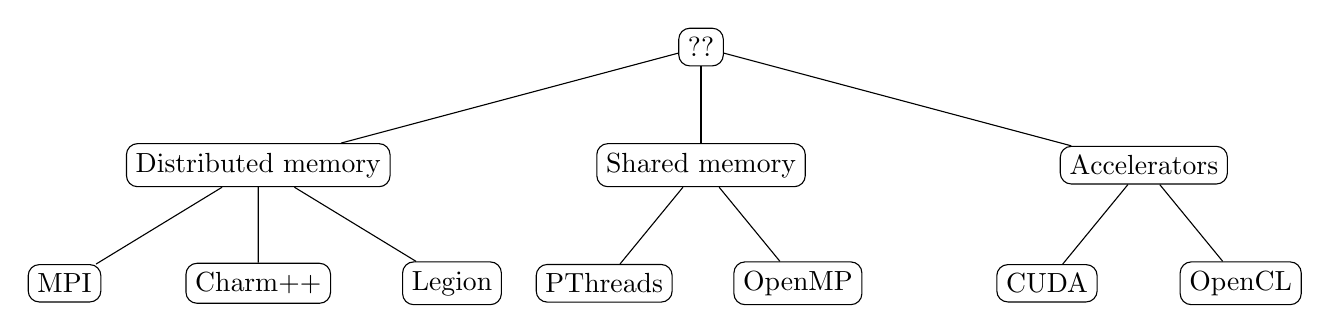
\begin{tikzpicture}[
  every node/.style = {
    level distance=1em,
    shape=rectangle, 
    rounded corners,
    draw, 
    align=center,
    top color=white%, 
   % bottom color=blue!20
  }]]
  \node {??} [sibling distance=16em]
    child { node {Distributed memory} [sibling distance=7em]
        child{node {MPI}} 
        child{node {Charm++}}
        child{node {Legion}}
    }
    child { node {Shared memory} [sibling distance=7em]
      child { node {PThreads}}
      child { node {OpenMP}}
    }
    child { node {Accelerators} [sibling distance=7em]
      child {node  {CUDA}} 
      child { node {OpenCL}}
    };
\end{tikzpicture}
\caption{MIMD memory models}
\label{fig:1_HPC:mimd_memory_model}
\end{figure}

The runtimes, libraries and API we describe can be use in combination. 
The usual one is MPI for distribution, OpenMP and CUDA to target GPUs. 

\section{Benchmark}

This section regroup a bunch of the most famous nowadays benchmarks for HPC. 

\subsection{TOP500}
The most famous benchmark is certainly the TOP500\footnote{http://www.top500.org}. 
It gives the ranking of the 500 most powerful, known, supercomputers of the world as its name indicates.
Since 1993 the organization assembles and maintains this list updated twice a year in June and November.

This benchmark is based on the LINPACK\cite{dongarra1994top500} a benchmark introduced by Jack J. Dongarra.
This benchmark rely on solving  dense system of linear equations. 
As specified in this document this benchmark is just one of the tools to define the performance of a supercomputer. 
It reflects "the performance of a dedicated system for solving a dense system of linear equations".
This kind of benchmark is very regular in computation giving high results for FLOPS. 

\subsection{GREEN500}
In conjunction of the TOP500, the GREEN500 focus on the energy consumption of supercomputers. 
The scale is based on FLOPS per watts~\cite{feng2007green500}.

\subsection{GRAPH500}
The GRAPH500 benchmark focus on irregular memory accesses, and communications.
It will be detailed in Part. II Chapter II in our benchmark suite. 


\section{Conclusion}


